\chapter{Erstes Kapitel}
\label{kap:eins}
Dies ist eine Vorlage für wissenschaftliche Arbeiten an der FHGR nach \textcite{selina_leitfaden_nodate}. Nachfolgend einige Tipps und Funktionen, welche in der Vorlage enthalten sind.

\section{Glossar und Abkürzungen}
Mit den Befehlen \setminus acrlong\{zb\}, \setminus acrshort\{zb\} oder \setminus acrfull\{zb\} ist das Ausgeben der im Dokument conten/00\_assets/01\_Vorspann/01.4\_abkuerzungsverzeichnis\_glossar.tex Einträgen möglich: \acrlong{zb}, \acrshort{zb}, \acrfull{zb}.

\section{Zitieren}
Für das Zitieren wird die Erweiterung BibLaTeX verwendet. Sämtliche Befehle und Funktionen des Pakets können im Handbuch nachgeschlagen werden\footnote{https://mirror.metanet.ch/tex-archive/info/translations/biblatex/de/biblatex-de-Benutzerhandbuch.pdf}. Voraussetzung ist, dass die Quellen erst im BibLaTeX Format unter content/00\_assets/quellen.bib abgelegt sind (z. B. via Zotero, Mendely oder als Datei). Nachfolgend Beispiele mit den üblichsten Befehlen:\\
\\
\setminus textcite\{diani\_black\_2016\} gibt als Ausgabe:\\ 
\textcite{diani_black_2016}\\
\\
\setminus parencite\{diani\_black\_2016\} gibt als Ausgabe:\\ 
\parencite{diani_black_2016}\\
\\
\setminus parencites[S. 10]\{diani\_black\_2016\}[S. 20]\{selina\_leitfaden\_nodate\} gibt als Ausgabe:\\ 
\parencites[S. 10]{diani_black_2016}[S. 20]{selina_leitfaden_nodate}\\
\\
Zusätzlich stehen die folgenden eigens im Template definierten Befehle zur Verfügung:\\
\\
\setminus parenciteabbr\{org\_2022\}\{orln\} gibt als Ausgabe:\\ 
\parenciteabbr{org_2022}{orln}\\
\\
\setminus textciteabbr\{org\_2022\}\{orln\} gibt als Ausgabe:\\ 
\textciteabbr{org_2022}{orln}\\
\\
Zur Formatierung eines Blockzitats kann der Befehl \setminus begin\{quote\} ... \setminus end\{quote\} verwendet werden:
\begin{quote}
Blockzitate sind wörtliche Zitate von 40 Wörtern oder mehr; sie werden als eigener Absatz ohne Anführungszeichen angeführt.
Ein Blockzitat beginnt stets in einer neuen Zeile, wird zur Gänze (also jede Zeile) 1,3 cm oder fünf Leerschritte eingerückt und mit zweizeiligem Abstand geschrieben. Absätze innerhalb eines Blockzitates werden vom neuen Rand des Blockzitates eingerückt. Blockzitate werden nicht in Anführungszeichen gesetzt, darin aufscheinende Zitate werden in doppelten Anführungszeichen wiedergegeben. Die Quellenangabe am Ende eines Blockzitates steht nach dem letzten schließenden Punkt des Zitates in Klammern gesetzt, danach folgt kein weiterer Punkt. \parencite[S. 111]{psychologie_richtlinien_2016}
\end{quote}

\chapter{Ein Bild}
\begin{figure}[H]
    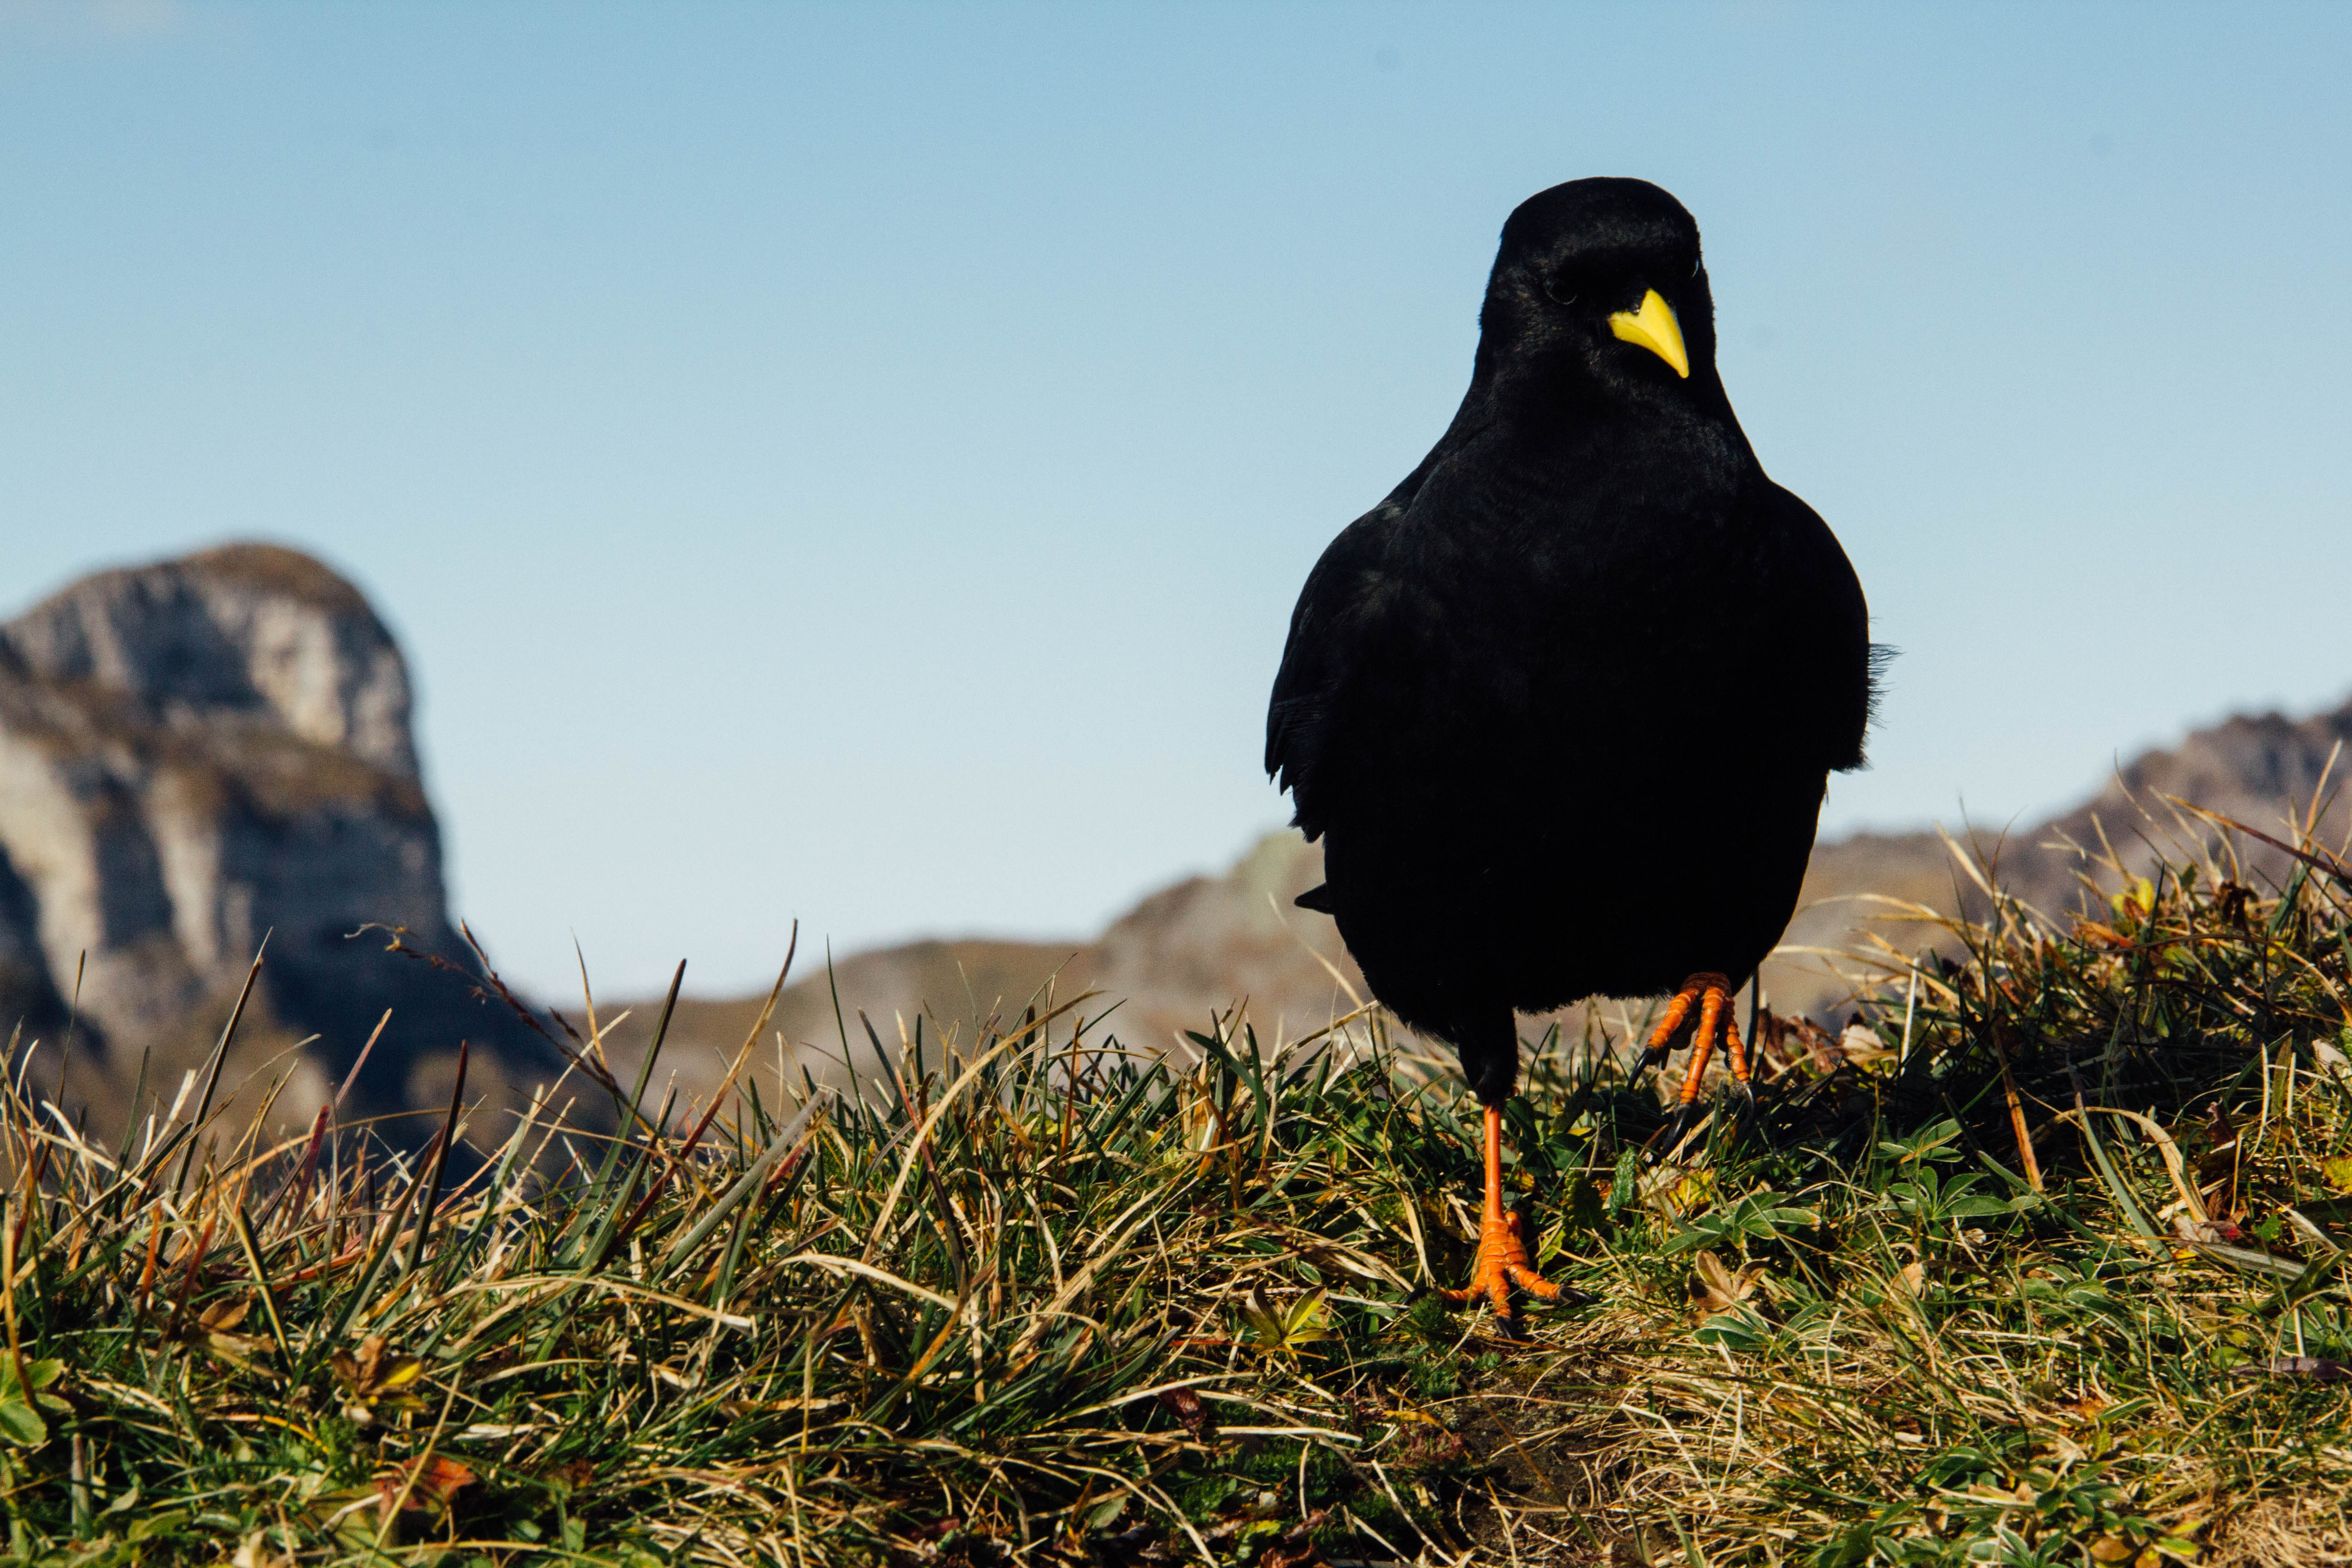
\includegraphics[width=\textwidth]{alpendohle.jpg}
    \caption{Eine Alpendohle \parencite{diani_black_2016}}
    \label{fig:alpendohle}
\end{figure}

\chapter{Tabelle}
Das folgende Beispiel zeit eine Tabelle:
\begin{table}[ht]
\begin{tabularx}{\textwidth} {
    >{\raggedright\arraybackslash}X 
    >{\raggedleft\arraybackslash}X 
    >{\raggedleft\arraybackslash}X}
        \hline
        \multicolumn{3}{c}{\textbf{Tabelle}}\\
        \hline
        \textbf{Linksbündig} & \textbf{Rechtsbündig} & \textbf{Rechtsbündig}\\
        \hline
        Lorem & N/A & N/A\\
        Ipsum & 1 499 & 8 512\\
        Dolor & 297 & N/A\\
        Sit & 1 053 & N/A\\
        \hline
        \textbf{Total} & 2 849 & 8 512\\
        \hline
\end{tabularx}
\caption{Beispiel einer Tabelle.}
    \label{tab:tabelle}
\end{table}